\begin{apendicesenv}
    \newpage
    \phantomsection
    \addcontentsline{toc}{chapter}{APÊNDICES}
    \addtocontents{toc}{\protect\setcounter{tocdepth}{-1}}

    \chapter{Organização e acesso ao repositório do projeto}
    \label{ap:repositorio}

    O repositório \textit{Quadcopter AeroRoute} reúne o código-fonte, a documentação técnica e os arquivos LaTeX desenvolvidos neste trabalho. Sua organização acompanha a divisão da plataforma entre o controlador de voo STM32 e o computador de missão Raspberry Pi, permitindo identificar as responsabilidades de cada componente e consultar os materiais de apoio à continuidade do projeto. O endereço do repositório é:

    \begin{center}
        \url{https://github.com/rickelmedias/Quadcopter-AeroRoute}
    \end{center}

    O diretório \texttt{stm32/} contém o projeto do \textit{firmware} do controlador de voo. Seus principais diretórios são:

    \begin{alineastcc}
        \item \texttt{App/}: implementação das funções da aplicação, incluindo aquisição de sensores, estimação de estados, controle, execução dos comandos de voo e funções locais de segurança;
        \item \texttt{protocol/}: definição das mensagens do protocolo DroneLink, que estabelece a interface de comunicação entre o controlador de voo e o computador de missão;
        \item \texttt{tools/}: ferramentas de apoio ao desenvolvimento e à preparação do \textit{firmware};
        \item \texttt{docs/}: documentação técnica e registros do projeto disponibilizados para consulta.
    \end{alineastcc}

    O diretório \texttt{raspberry/} contém o software do computador de missão, responsável pelo planejamento e pela coordenação da execução das rotas, pela comunicação com o STM32 e pela interface de comandos do operador. Além de calcular a ordem de visita aos pontos, esse software transforma a rota em uma sequência de comandos de movimento, acompanha as respostas do controlador de voo e envia o próximo trecho somente após a confirmação de conclusão do anterior. O STM32 permanece responsável pela validação dos pedidos, pela execução dos movimentos, pela estabilização e pelas funções locais de segurança.

    O diretório \texttt{latex/} reúne os arquivos-fonte deste trabalho, incluindo os capítulos, as referências bibliográficas e as figuras utilizadas na composição do documento.

    Essa organização permite consultar separadamente a implementação embarcada, a coordenação das missões e a descrição acadêmica do projeto. Como o código pode receber atualizações após a conclusão do trabalho, a reprodução de um ensaio deve considerar a versão do software e os parâmetros associados ao respectivo registro experimental.

    \chapter{Esquema de ligação do protótipo}
    \label{ap:diagrama_ligacao}

    A Figura~\ref{fig:diagrama_ligacao} apresenta o esquema de interligação elétrica do protótipo, com a distribuição de alimentação e as conexões entre o STM32F411, o Raspberry Pi Zero W, os sensores, o ESC e os motores. Os sinais de comunicação e os pinos indicados permitem relacionar a montagem física às interfaces descritas na metodologia.

    \begin{figure}[p]
        \centering
        \caption{Esquema de ligação elétrica do protótipo.}
        \label{fig:diagrama_ligacao}
        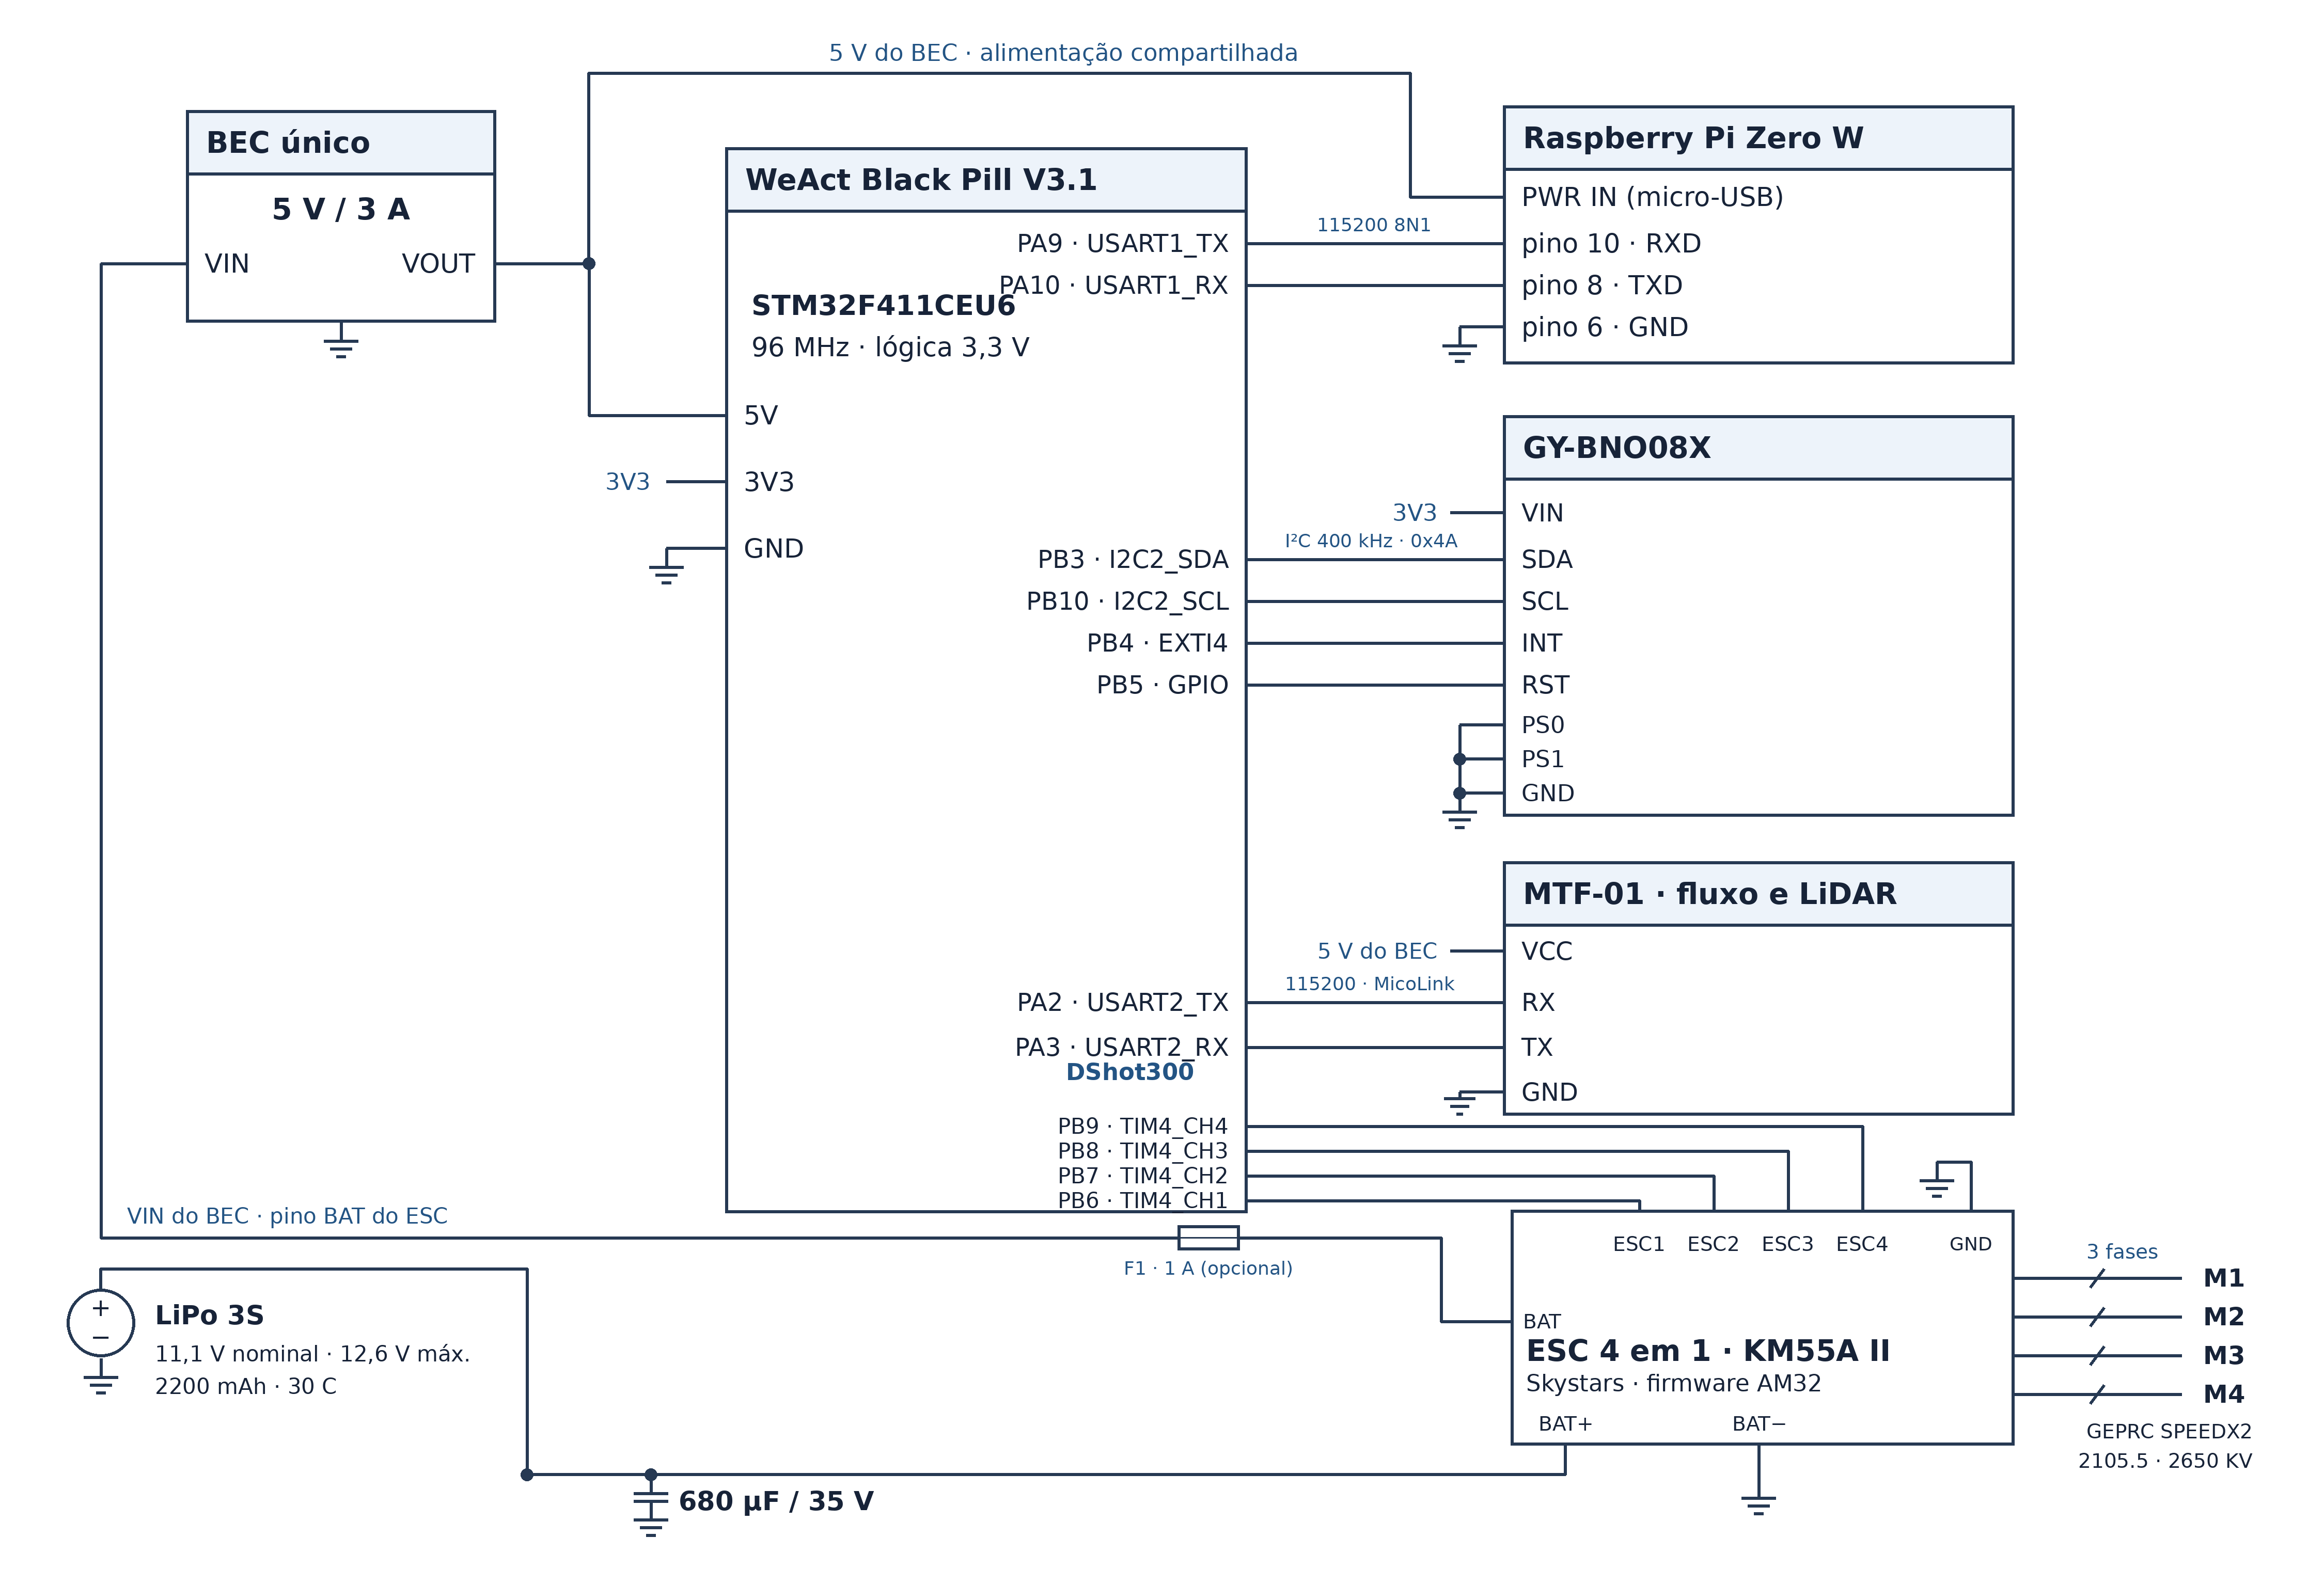
\includegraphics[width=\textwidth,height=0.85\textheight,keepaspectratio]{images/apendices/diagrama_eletrico.png}
        \par\vspace{0.2cm}
        \footnotesize Fonte: elaborado pelos autores (2026).
    \end{figure}
    \clearpage

    \addtocontents{toc}{\protect\setcounter{tocdepth}{0}}
\end{apendicesenv}
